% Yiyong Sun,yiyognhit@gmail.com,2017.03.05 %% The current version should be listed at the first sight. Any changes, mark your name mailbox and the date
\newcommand{\CurrentDate}{05,03,2017}
\documentclass[a4paper,12pt,UTF8]{article}


\usepackage{CJKutf8}
\usepackage{amsfonts}
\usepackage{amsmath}
\usepackage{mathrsfs}
\usepackage{latexsym}
\usepackage{graphicx}
\usepackage{cite}
\usepackage[dvipdfmx,unicode,           %dvi-->pdf ????
            bookmarksnumbered=true]{hyperref}
\newtheorem{remark}{注解}

\begin{CJK}{UTF8}{gkai} % {gkai}{gbsn}

\begin{document}

\title{SMT数据统计规范}
\author{高会军,孙一勇,马志强,李政凯
\thanks{\textbf{哈尔滨工业大学智能控制与系统研究所}}
\date{\CurrentDate} % Curent Date
}
\maketitle


\section{总则}
目的:规范,未来方便生成各类报表、图表。统一文件路径、数据命名格式等。

\begin{figure}%[tbph]
\centering
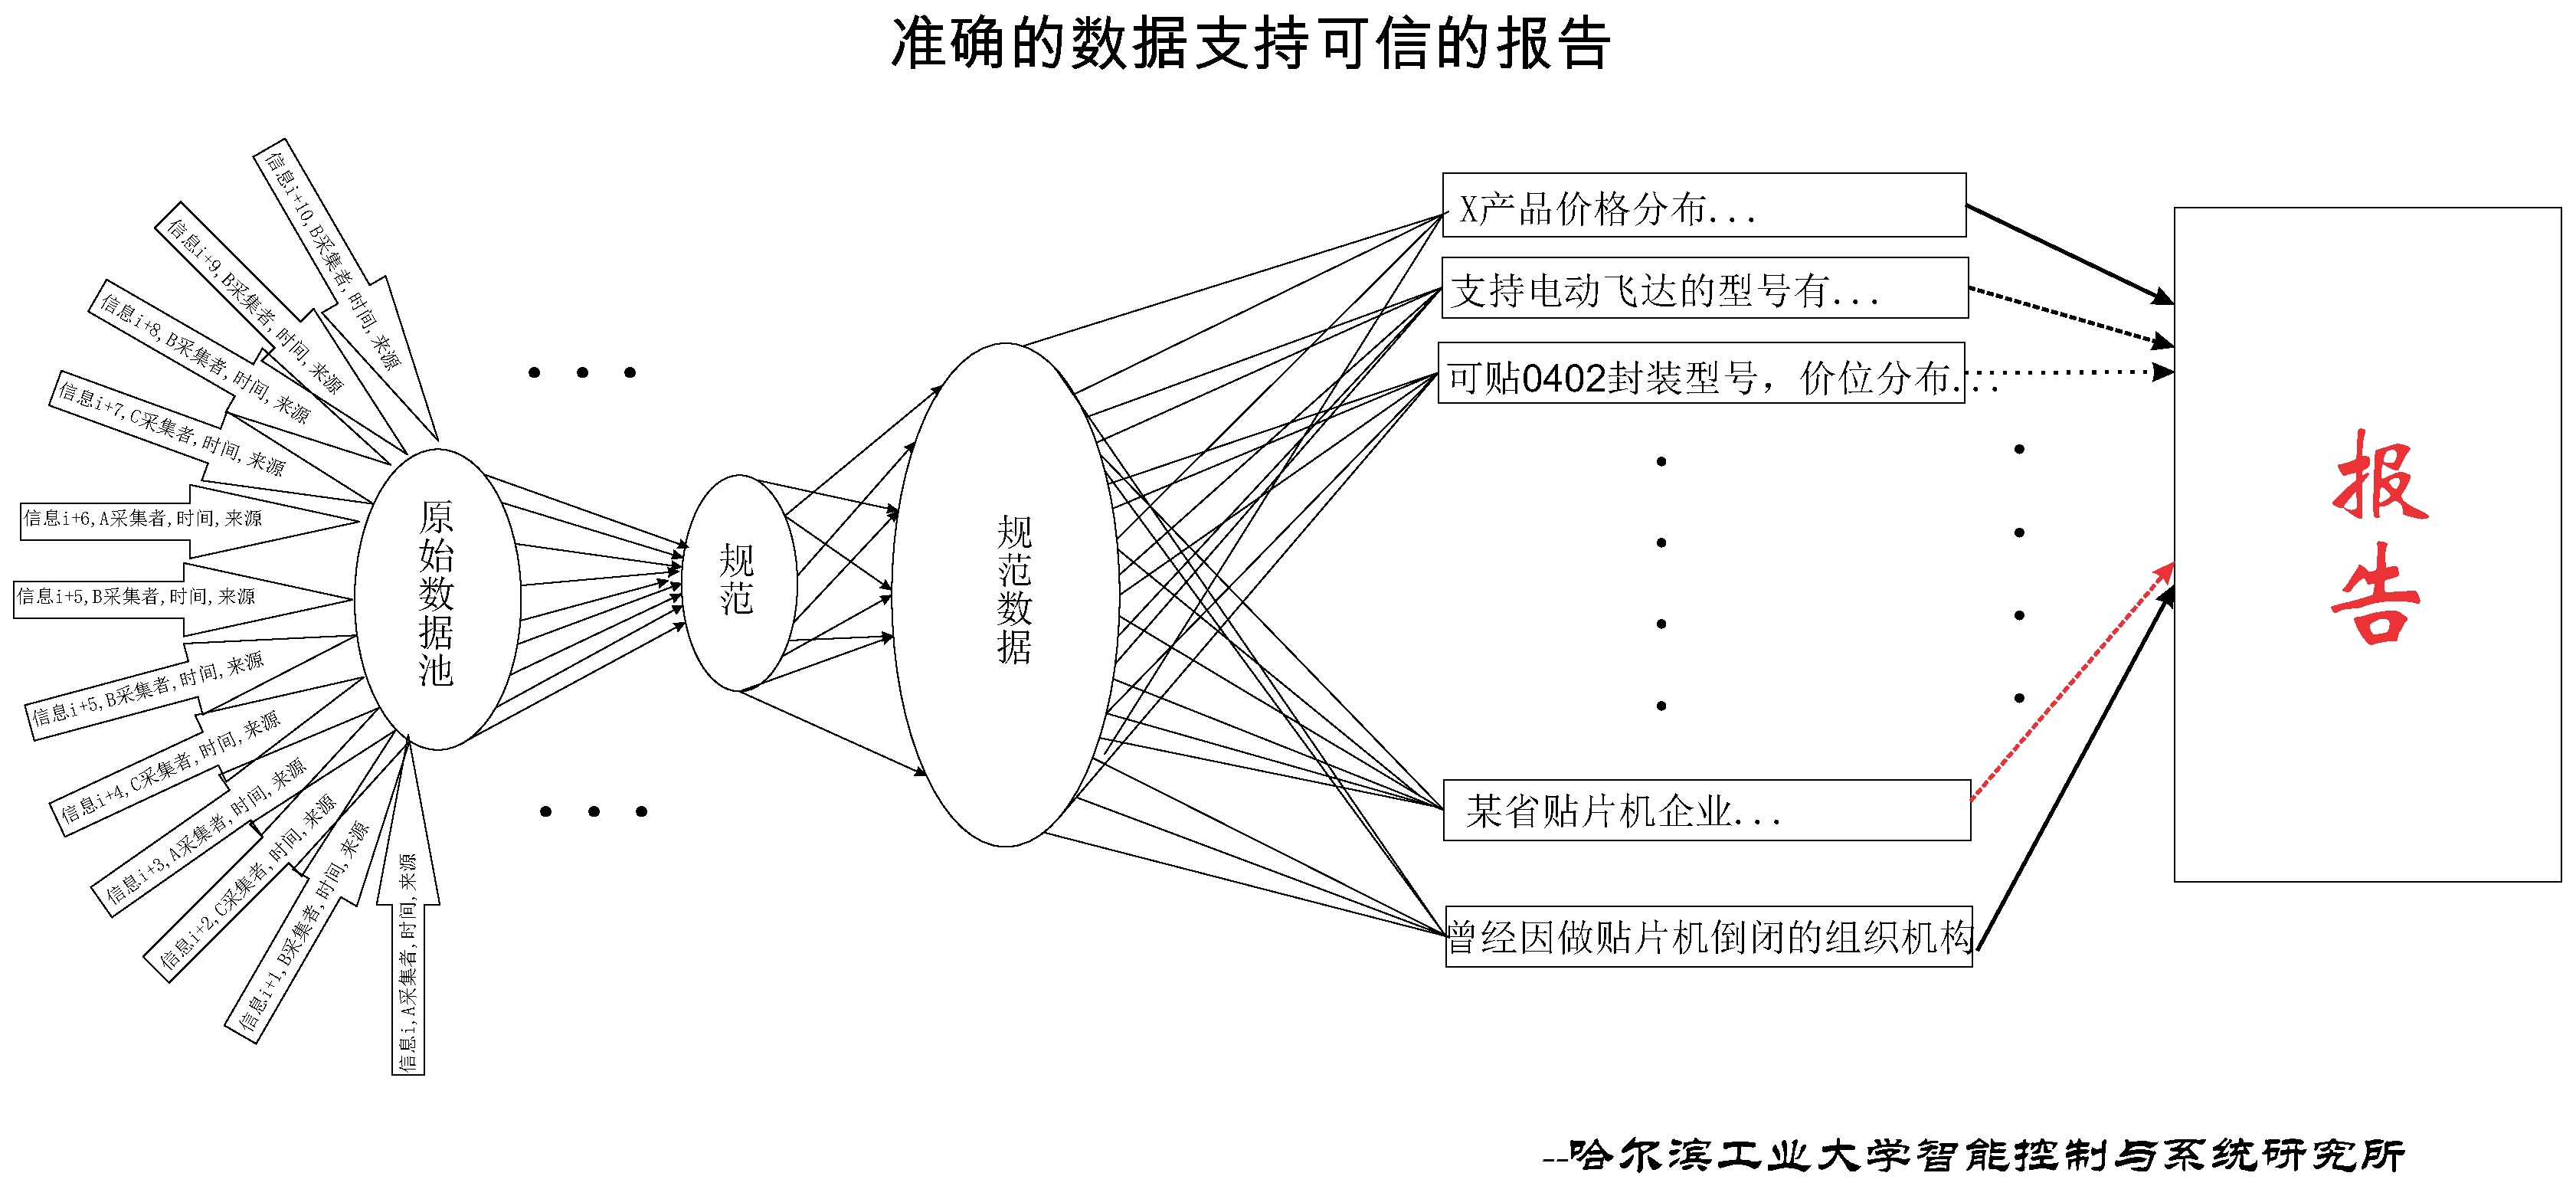
\includegraphics[width=13.1cm,height=7cm]{SMT_Report_2017.03.10.eps}
\caption{整体结构}
\label{FigLabel_Section1_StructurePicture}
\end{figure}


统计内容纷繁庞杂,未来统计目的不甚明确,需要有利与我的报告。由于所统计数据包罗各个行业各个领域,仅作粗略数据采集难以满足后期数据统计和处理需要: 以国内贴片机为例,现有数据中至少30+ 企业、10+研究机构和高校正在从事(或从事过)贴片机研发和生产相关的项目,其中仅产品型号一项至少有200 项之多。鉴于此,特制定本规范对数据管理、命名进行规则化处理。数据命名须尽量遵循以下原则:
\begin{itemize}
  \item 1:利于软件调用、方便生成各类格式的图表,每个厂家(组织)、每个型号的信息作为数据库的一部分,统一格式命名,各自对应其数据,有条不紊,
       比如:1)统计现有数据库中海外型号贴片机中日本厂家,能够很快地得出一共有N家,包括有松下、JUKI...等数据; 2)统计现有国内贴片机中支持电动飞达的厂家,通过查询数据就可以极快调动出现有数据库中此类厂家名称、支持的型号有哪些;
  \item 2:方便拓展,能够及时对现有的数据库做出补充,
        比如:1)某厂家2016年面世一款型号产品,现有数据库中并没有囊括这类型号,一旦发现可以及时添加此类信息,并能够统计这类数据的来源; 2)已知某不完整或不可信数据,那么须对该数据已知部分进行统计,未统计到部分可为空。
  \item 3:分类尽量完整,数据中可以反映一些联系,
        比如:1)现有统计数据中仅有贴片机厂家,不包含某研究机构或高校,发现H高校和A企业正在合作(或曾经合作过),高校和企业属于并列关系,通过查询H 高校就可以查找出H高校和A企业的合作关系; 2) A企业和B企业都在使用某S外企的软件界面、J企业的飞达、可与L企业的优化软件进行联调,但A企业与W企业的后端产品由于机械尺寸、软件环境等原因不能进行联合使用,发现这类信息,分别添加到A、S、J、W企业的相关产品信息下。
  \item 4:本规范为所有数据的地图,通过查询本数据规范,可以直接知道如何调用任一数据,比如数据格式为: 外企-美国-A企业-A1高速机-0.05mm精度;A2中速机-0.04mm精度;A3低速机- 高精度,大片,0.001mm精度 等几类型号:A1:仅支持电动飞达...。查询时通过下表快速即可以知道如何获取A企业的A22型号的所有信息。即表可以看出任意一个点上数据的调用方式。
  \item 5:考虑通性,所有企业共有的一些数据在同类中进行命名时须尽量使用同一命名方式,方便数据读写和更改。 比如: A、B、C企业均为外企,D、E、F企业均为国内民企, 那么他们的员工结构(-02)、某类产品(-08)在这些企业下的子类须为同一格式,即,员工结构分别为 国外-地域-A (或B 或C)-02,国内-地域-D(或 E 或 F)-02, 改类产品分别为 国外-地域-A (或B 或C)-08,国内-地域-D(或 E 或 F)-08。
\end{itemize}



\section{贴片机数据格式规范}
数据格式:一级,二级,三级...

数据编号格式:国内外 -- 地域 (所在城市) -- 公司、研究机构 -- 产品内容、人员结构 -- LED专用贴片机、泛用机、快速机、桌面机 -- 贴片机数据 -- 数据子类

贴片机数据包括:
机器型号、重量、价格、精度、速度、机械结构、传动结构、喂料器、气源、电源、贴装尺寸、

贴片机:LED贴片机、泛用机,贴插机,国内、国外,

\begin{remark}
\textbf{CC}-当前待确定数据, \textbf{XX-}或者数字代表当前已经确立数据。
\end{remark}

\textbf{{CC-}} 国内外:
\begin{itemize}
  \item 00未知%
  \item 01国外%
  \item 02国内%
  \item ...
\end{itemize}

地域:(主要是产品对应公司所在地,比如A集团B公司的产品进行调研,以B公司的所在地为准)

\textbf{01-CC} 国外分类
\begin{itemize}
  \item 00未知%
  \item 01德国%
  \item 02美国%
  \item 03日本%
  \item 04新加坡
  \item ...
\end{itemize}

\textbf{02-CC} 国内分类
\begin{itemize}
  \item 00未知%
  \item 01中国台湾
  \item 02深圳
  \item 03广州
  \item 04北京
  \item 05苏州
  \item 06杭州
  \item 07哈尔滨
  \item ...
\end{itemize}


\textbf{XX-XX-CC}组织性质: 主要是指该公司或者团体的性质
\begin{itemize}
  \item 00未知%
  \item 01上市公司
  \item 02公司
  \item 03研究所
  \item 04高校
  \item 05学术团体
  \item 06民间组织
  \item ...
\end{itemize}

\textbf{XX-XX-XX-CC} 考察内容
被统计内容性质:(主要是产品对应的属性)
\begin{itemize}
  \item 00未知%
  \item 01研究报告%
  \item 02专利和论文%
  \item 03软件
  \item 04贴片机
  \item 05丝印机
  \item 06接驳台
  \item 07外围产品(飞达、焊锡、焊锡膏)
  \item 08波峰焊台
  \item 09机器人
  \item 10机构历史
  \item 11组织规模
  \item 12人员结构
  \item 13机构资金
  \item ...
\end{itemize}

\textbf{XX-XX-XX-04-CC} 贴片机
\begin{itemize}
  \item 00未知%
  \item 01注册资金
  \item 02销售额
  \item 03研发资金
  \item 04盈利情况
  \item ...
\end{itemize}

\textbf{XX-XX-02-04-XX-CC} 某公司、某型号贴片机的参数
\begin{itemize}
  \item 00未知%
  \item 02重量
  \item 03价格
  \item 04精度
  \item 05速度
  \item 06机械结构
  \item 07喂料器
  \item 08气源
  \item 09电源
  \item 10机器类型
  \item 11相机类型
  \item 12贴装原件(尺寸、最小及最大类型)
  \item 13可连外围设备(其他贴片机 接驳台)
  \item 14计算机结构(是否支持联网、分布式)
  \item 15操作系统(XP、Linux等 语言)
  \item 16软件可定制化程度(细节信息的可设定调整性能)
  \item 17连续工作时间
  \item ...
\end{itemize}

\textbf{XX-XX-XX-04-xx-06-CC} 某型号贴片机机械结构
\begin{itemize}
  \item 00未知%
  \item 01头部结构 (转盘式、动臂式、复合式、大型平行系统、吸杆数)
  \item 02传送带(段数 可否移动)
  \item 03XY传动结构(丝杠 直线电机 皮带 悬臂个数)
  \item 04贴装pcb面积(Xmax Xmin  Ymax Ymin)
  \item 05整机尺寸(长、宽、高)
  \item ...
\end{itemize}

\textbf{XX-XX-XX-04-xx-07-CC} 某型号贴片机喂料器支持情况
\begin{itemize}
  \item 00未知%
  \item 01是否支持电动
  \item 02是否支持气动
  \item 03基座是否可动
  \item 04数量
  \item 05是否支持飞达车
  \item ...
\end{itemize}

\textbf{XX-XX-XX-04-xx-08-CC} 外接气源情况
\begin{itemize}
  \item 00未知%
  \item 01可不需要外接气源
  \item 02必须外接气源
  \item 03气动飞达外接气源
  \item ...
\end{itemize}

\textbf{XX-XX-XX-04-xx-09-CC} 外接电源情况
\begin{itemize}
  \item 00 未知%
  \item 01 110V-60hz
  \item 02 220V-50hz
  \item 03 兼容
  \item 04 三相、单相
  \item ...
\end{itemize}

\textbf{XX-XX-XX-04-xx-11-CC} 需要相机类型
\begin{itemize}
  \item 00未知%
  \item 01CCD面阵相机
  \item 02CCD线扫相机
  \item 03镭射
  \item 04有无飞行相机
  \item 05固定相机
  \item 06基准相机
  \item ...
\end{itemize}

\textbf{XX-XX-XX-04-xx-10-CC} 机器类型
\begin{itemize}
  \item 00未知%
  \item 01LED专用贴片机
  \item 02泛用机
  \item 03贴插机
  \item ...
\end{itemize}




\textbf{XX-XX-XX-12-CC} 人员结构
\begin{itemize}
  \item 00未知%
  \item 01总人数
  \item 02研究人员总量
  \item 03研究人员比例(博-硕-本-高中及以下)
  \item ...
\end{itemize}

\textbf{XX-XX-XX-13-CC} 机构资金
\begin{itemize}
  \item 00未知%
  \item 01注册资金
  \item 02销售额
  \item 03研发资金
  \item 04盈利情况
  \item ...
\end{itemize}

\section{信息来源}
每条信息都有其一定的可信程度,在数据统计过程中不对其置信程度做任何评价,但是要对每一条信息的来源进行说明。仅作信息收集,不做信息处理。如此,一方面保证信息数据库的包容性,另一方面对信息后期处理进行一定程度的置信分析。 同时,原始数据应当保留在另外一个库中,注明数据收集人姓名。

比如: 有关A组织机构现有200条信息,其中100条是通过网站、口述得到的,另外100条是通过该组织机构的宣传海报、专利授权、网站等内容获得的。在整理报告时,可以对两部分数据进行差别统计和处理。

信息来源:
\begin{itemize}
  \item 00未知%
  \item 01同上一级%
  \item 02公司网站%
  \item 03电话%
  \item 04听人口述%
  \item 05文献资料%
  \item ...
\end{itemize}
\begin{remark}
所有信息来源的文献、网站、以及可再次获取的信息,须在文末以参考资料的形式给出。尽量做到数据可多次复查、禁得住查。 比如,某品牌产品在某论坛口碑不佳、易损,统计此类信息时,则是该品牌的口碑信息之一,在参考资料一项中需给出其评价信息的网页链接。
\end{remark}
\end{CJK}
\end{document}

%This file should be compiled with latex!!!
